%%%%%%%%%%%%%%%%%%%%%%%%%%%%%%%%%%%%%%%%%%%%%%%%%%%%%%%%%%%%%%%%%
%
% chapter_example.tex
%
% contains an example of the common elements found in a chapter
%
%
%%%%%%%%%%%%%%%%%%%%%%%%%%%%%%%%%%%%%%%%%%%%%%%%%%%%%%%%%%%%%%%%%

% DOCUMENT STRUCTURE
\chapter{Chapter Example} \label{ch:example}   		% chapter title i.e. 1

\section{blah}	\label{sec:example}			% section header i.e. 1.1
Lorem ipsum dolor sit amet, consectetur adipiscing elit. Praesent suscipit nisi ligula, vitae dignissim magna egestas et. Donec id augue dolor. Morbi aliquet diam turpis, ut molestie est ornare nec. Nulla ullamcorper libero quis nibh aliquam tempor. Nam viverra consequat ullamcorper. Duis sed ullamcorper nisl. Integer scelerisque imperdiet massa nec feugiat. Duis faucibus accumsan eros vel porta. Aliquam erat volutpat. Praesent ultrices tellus et convallis consectetur. Nullam ullamcorper, dolor varius placerat convallis, mauris massa tristique urna, ut ornare arcu magna ac erat. Sed tempus eu mi eu porta. Curabitur dolor turpis, volutpat vel placerat ac, accumsan vitae mauris. In mattis ante sem, quis imperdiet ligula laoreet eget. Etiam ut fringilla nibh, a feugiat orci.


\subsection{more blah}						% next level section i.e. 1.1.1
Lorem ipsum dolor sit amet, consectetur adipiscing elit. Praesent suscipit nisi ligula, vitae dignissim magna egestas et. Donec id augue dolor. Morbi aliquet diam turpis, ut molestie est ornare nec. Nulla ullamcorper libero quis nibh aliquam tempor. Nam viverra consequat ullamcorper. Duis sed ullamcorper nisl. Integer scelerisque imperdiet massa nec feugiat. Duis faucibus accumsan eros vel porta. Aliquam erat volutpat. Praesent ultrices tellus et convallis consectetur. Nullam ullamcorper, dolor varius placerat convallis, mauris massa tristique urna, ut ornare arcu magna ac erat. Sed tempus eu mi eu porta. Curabitur dolor turpis, volutpat vel placerat ac, accumsan vitae mauris. In mattis ante sem, quis imperdiet ligula laoreet eget. Etiam ut fringilla nibh, a feugiat orci.


\subsubsection{even more blah}				% another level section i.e. 1.1.1.1
Lorem ipsum dolor sit amet, consectetur adipiscing elit. Praesent suscipit nisi ligula, vitae dignissim magna egestas et. Donec id augue dolor. Morbi aliquet diam turpis, ut molestie est ornare nec. Nulla ullamcorper libero quis nibh aliquam tempor. Nam viverra consequat ullamcorper. Duis sed ullamcorper nisl. Integer scelerisque imperdiet massa nec feugiat. Duis faucibus accumsan eros vel porta. Aliquam erat volutpat. Praesent ultrices tellus et convallis consectetur. Nullam ullamcorper, dolor varius placerat convallis, mauris massa tristique urna, ut ornare arcu magna ac erat. Sed tempus eu mi eu porta. Curabitur dolor turpis, volutpat vel placerat ac, accumsan vitae mauris. In mattis ante sem, quis imperdiet ligula laoreet eget. Etiam ut fringilla nibh, a feugiat orci.


% FIGURES
\begin{figure}[t]
\centering
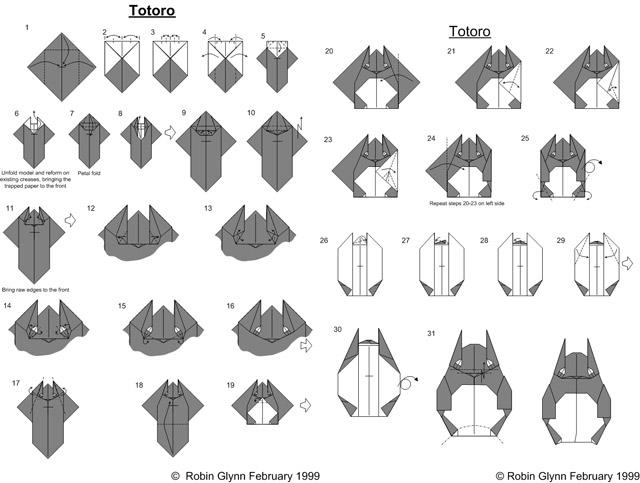
\includegraphics[scale=0.6]{./fig/totoro-origami.jpg}
\caption[Figure caption entry for list of figures]{Figure Caption}
\label{fig:example}		
\end{figure}

% TABLES
% if you have text that needs wrapping, use p{5cm}, in place of l c or r, to set a column width.  Vary the width to find one that fits 

% a small table can often be fitted whole into a file:
\begin{table}[t]
\centering
\caption[Table caption entry for list of tables]{Table Caption}
\label{tab:example1}
\begin{tabular}{lc}
\hline
\textbf{Year} & \textbf{Film Title} \\
\hline
1988 & Grave of the Fireflies \\
1988 & My Neighbour Totoro \\
1994 & Pom Poko \\
2001 & Spirited Away \\
2014 & The Wind Rises \\
\hline
\end{tabular}
\end{table}

% if a table is much larger you can call it from a different file:
\begin{table}[t]
\centering
\caption[Table caption entry for list of tables]{Table Caption}
\label{tab:example2}
\begin{tabular}{lc}
\hline
\textbf{Fact} & \textbf{Statistic} \\
\hline
My Neighbour Totoro IMDb rating & 8.2 \\
Japan Academy Prizes & 3 \\
Number of feature films & 20 \\
Years since founded & 28 \\
Employees & 300 \\
\hline
\end{tabular}  % this reads in an ugly file containing everything in the tabular environment
\end{table}


% EQUATIONS
\begin{equation} \label{eq:example}
E=mc^{2}
\end{equation}

\begin{equation} \label{eq:calculus}
\frac{df}{dt}=\lim_{h\to0}\frac{f(t+h)-f(t)}{h}
\end{equation}

Inline equations can also be used in the text using dollar signs e.g. $H=-\sum p(x) logp(x)$.

% REFERRING TO FIGURE/TABLE/SECTION/EQUATION LABELS

Use labels to refer to automatic numbering such as with Figure \ref{fig:example}, Table \ref{tab:example1} whilst Tables \ref{tab:example1} and \ref{tab:example2} can be referred to like this which are all found in Chapter \ref{ch:example}.

% CITATIONS
Citation in parantheses: \citep{Soo2011}

Citation in text: \citet{Greenberg2012}

Multiple citations: \citep{Soo2011,Suctani2011,Greenberg2012}







	

